
Throughout the paper, we always assume that matrix monoids are defined by sets of generators, and 
all matrices are square zero-one unless stated otherwise.

\subsection{Total DFAs}

An $n \times n$ zero-one matrix with exactly one $1$ in every row can be equivalently seen as a transformation of a set $Q$ of size $n$. A set of such matrices generates a zero-one matrix monoid, and can be seen as a total deterministic finite (semi-)automaton\footnote{\label{footnote-semi}In this paper, all automata are semi-automata, meaning that they do not have any initial or accepting states, and thus do not recognise any languages. Following the usual conventions (as in, e.g.,~\cite{Berstel2010}), we omit ``semi-'', in particular because it would make abbreviations like DFA less recognisable. Total DFAs are often called complete, but we prefer the
term “total” both to avoid the clash of terminology with complete UFAs and because of the obvious connection
with total functions.} (total DFA) $\Aa = (Q, \Sigma, \delta)$. Here, $\Sigma$ is a finite alphabet whose letters correspond to the generating matrices, and $\delta: Q \times \Sigma \to Q$ is the transition function defined in such a way that for each $a \in \Sigma$, $\delta(\underline{\hspace{0.25cm}}, a)$ is the transformation of $Q$ induced in the natural way by the matrix corresponding to $a$. Thus, words over $\Sigma$ correspond to products of the generating matrices.

The \emph{rank} of a word $w$ in $\Aa$ is the size of the image of $Q$ under the transformation corresponding to $w$. Equivalently, it is the real rank of the matrix corresponding to $w$.
The \emph{rank} of a total DFA is the minimum among the ranks of all its words. This concept was studied from the perspectives of automata theory \cite{Rystsov1992Rank,Kari2019} and the theory of transformation semigroups \cite{Shin2010Rank,Karimi2017MinIdeal}. It is the subject of the rank conjecture (called the \v{C}ern\'{y}-Pin conjecture in \cite{Rystsov1992Rank}), which states that every total DFA of rank $r$ admits a word of rank $r$ having length at most $(n - r)^2$. The \v{C}ern\'{y} conjecture, one of the oldest open problems in combinatorial automata theory \cite{Volkov2022}, is a special case with $r = 1$. We refer to surveys \cite{Volkov2008,Beal2016,Kari2019,Volkov2022} for the vast literature on the \v{C}ern\'{y} conjecture. Underlying digraphs of total DFAs of a given rank were studied in \cite{Budzban2011Generalized,Beal2016} in the context of the road colouring problem.

The rank of an $n$-state total DFA over an alphabet of size $m$ can be found in $\OO(m^4n^4)$ time \cite[Theorem 1]{Rystsov1992Rank}.
In contrast, for any fixed $r \ge 2$, the problem of checking if a total DFA admits a word of rank $r$ is \NP-hard~\cite{GORALCIK1995}. Checking if an $n$-state total DFA over an alphabet of size $m$ has rank one is \NL-complete \cite{Holzer2018,Volkov2022}, and can be done in $\OO(m n^2)$ time \cite{Eppstein1990,Volkov2008}. For each total DFA of rank $r$, there exists a word of rank $r$ of length at most $\frac{(n - r)^3}{6} + \OO((n - r)^2)$~\cite{Klyachko1987}, and if $r = 1$,  finding a word of rank one can be done in $\OO(n^3 + mn^2)$ time and $\OO(n^2)$ space~\cite{Eppstein1990}.

\subsection{Unambiguous finite automata}

Generalising the case of total DFAs, a set $\Aa$ of $n \times n$ zero-one matrices generating a zero-one matrix monoid can be equivalently seen as an unambiguous nondeterministic finite (semi-)automaton (UFA). Let $Q = \{q_1, \ldots, q_n\}$ be its set of states. To each matrix in $\Aa$ we again associate a letter in the alphabet $\Sigma$, and the transition relation $\Delta \subseteq Q \times \Sigma \times Q$ is defined so that $(q_i,a,q_j) \in \Delta$ if and only if the entry~$(i, j)$ in the matrix corresponding to $a$ is equal to one. Just as in the total DFA case, words over $\Sigma$ naturally correspond to products of matrices from $\Aa$.

The obtained NFA then has the property that is sometimes called \emph{diamond-free}: for every two states $p, q$ and every word~$w$, there is at most one path from $p$ to $q$ labelled by $w$. A simple reachability argument shows that the length of a shortest word labelling two such paths, if it exists, is at most quadratic in the dimension of the matrices. Hence, deciding whether an NFA is a UFA (and thus whether a set of zero-one matrices generates a zero-one monoid)  is in \coNL = \NL. It is actually \NL-complete as described in the next subsection.

A UFA is called complete if it does not admit a word whose matrix is the zero matrix. For an $n$-state UFA the length of such a word if it exists is at most~$n^5$~\cite{Kiefer2021}. 
The best known lower bound is quadratic in $n$, and is achieved by a series of DFAs~\cite{Rystsov1997}. 
For UFAs, the quadratic upper bound was conjectured to be tight~\cite[Conjecture 2]{Rystsov1992Rank}. Checking if a UFA is complete can be done in \NCT~\cite{Kiefer2021}. 

The \emph{real rank} of a UFA is the minimum among the real ranks of the matrices corresponding to words. It was shown in \cite{Carpi1988} that for an $n$-state UFA of real rank $r \ge 1$ there always exists a word of minimum rank of length $\OO(rn^3)$.
For $n$-state strongly connected Eulerian UFAs of rank one, a subclass with remarkably nice properties, there always exists a word of length at most $(n - 1)^2$ of rank one~\cite[Corollary~4]{Carpi2009}. All mentioned constructions also provide polynomial time algorithms that construct words with the required properties (in particular, with a length within the stated bounds).

\subsection{Applications to variable-length codes}\label{subs:var-length-codes}

A \emph{variable-length code} (or simply a \emph{code}) is a set $X$ of finite words over an alphabet $\Sigma$ such that every finite word over $\Sigma$ has at most one factorisation over $X$. In other words, a code is a basis of a free submonoid of $\Sigma^*$. 

The definitions of both UFAs and codes rely, intuitively, on the uniqueness of certain representations. In fact, UFAs and codes are tightly related. Let us illustrate this relationship.
If the cardinality of a code $X$ is finite, one can construct its flower automaton, which is a UFA with a chosen state $s$ such that, for each word from $X$, there is a separate cycle containing $s$ and labelled by this word, see \autoref{fig:flower} (left) for an example.
More generally, codes that are regular languages correspond precisely to strongly connected UFAs in a similar way, see \cite[Chapter 4]{Berstel2010} for the details.

\begin{figure}[h]
\centering
% Center the two drawings as a group
\begin{tabular}{@{}c@{\hspace{1cm}}c@{}}
\begin{tikzpicture} [node distance = 2cm]
%,
\tikzset{every state/.style={inner sep=1pt,minimum size=1.5em}}

\node [state] at (0, 0) (1) {$1$};
\node [state] at (-2, 0) (2) {$2$};
\node [state] at (-1, 1.5) (3) {$3$};
\node [state] at (1, 1.5) (4) {$4$};

\node [state] at (1.5, 0.75) (5) {$5$};
\node [state] at (1.5, -0.75) (6) {$6$};

\node [state] at (1, -1.5) (7) {$7$};
\node [state] at (0, -1.7) (8) {$8$};
\node [state] at (-1, -1.5) (9) {$9$};


\path [-stealth, thick]

(1) edge [bend left=30] node[above] {$a$} (2)
(2) edge [bend left=30] node[below] {$a$} (1)

(1) edge [bend left=10] node[right] {$a$} (3)
(3) edge [bend left=10] node[below] {$a$} (4)
(4) edge [bend left=10] node[left] {$b$} (1)

(1) edge [bend left=10] node[below] {$a$} (5)
(5) edge [bend left=10] node[left] {$b$} (6)
(6) edge [bend left=10] node[above] {$a$} (1)

(1) edge [bend left=10] node[left] {$a$} (7)
(7) edge [bend left=10] node[above] {$b$} (8)
(8) edge [bend left=10] node[above] {$a$} (9)
(9) edge [bend left=10] node[right] {$b$} (1)

;
\end{tikzpicture}
&
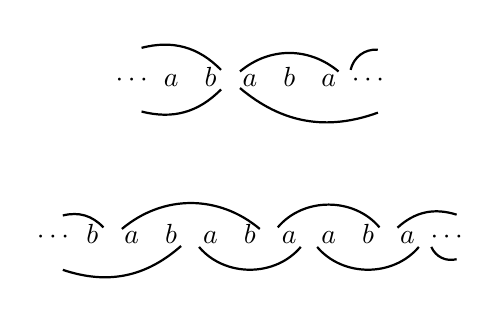
\begin{tikzpicture} [node distance = 2cm]

\node [] at (0.5, 2) (t0) {\strut $\cdots$};
\node [] at (0.5, 2.375) (t0u) {};
\node [] at (0.5, 1.625) (t0l) {};
\node [] at (1, 2) (t1) {\strut $a$};
\node [] at (1.5, 2) (t2) {\strut $b$};
\node [] at (1.75, 2) (t23) {};
\node [] at (2, 2) (t3) {\strut $a$};
\node [] at (2.5, 2) (t4) {\strut $b$};
\node [] at (3, 2) (t5) {\strut $a$};
\node [] at (3.25, 2) (t56) {};
\node [] at (3.75, 2.375) (t6u) {};
\node [] at (3.75, 1.625) (t6l) {};
\node [] at (3.5, 2) (0) {\strut $\cdots$};

%%%%%%%%%%%%%%%%%%%%%%
\node [] at (-0.5, 0) (0) {\strut $\cdots$};
\node [] at (-0.5, -0.375) (0l) {};
\node [] at (-0.5, 0.25) (0) {};
\node [] at (0, 0) (1) {\strut $b$};
\node [] at (0.25, 0) (12) {};
\node [] at (0.5, 0) (2) {\strut $a$};
\node [] at (0.75, 0) (23) {};
\node [] at (1, 0) (3) {\strut $b$};
\node [] at (1.25, 0) (34) {};
\node [] at (1.5, 0) (4) {\strut $a$};
\node [] at (1.75, 0) (45) {};
\node [] at (2, 0) (5) {\strut $b$};
\node [] at (2.25, 0) (56) {};
\node [] at (2.5, 0) (6) {\strut $a$};
\node [] at (2.75, 0) (67) {};
\node [] at (3, 0) (7) {\strut $a$};
\node [] at (3.25, 0) (78) {};
\node [] at (3.5, 0) (8) {\strut $b$};
\node [] at (3.75, 0) (89) {};
\node [] at (4, 0) (9) {\strut $a$};
\node [] at (4.75, 0.25) (10) {};
\node [] at (4.25, 0) (10l) {};
\node [] at (4.75, -0.25) (10ll) {};
\node [] at (4.5, 0) (11) {\strut $\cdots$};


\path [thick]

(t0u) edge [bend left=30] node[above] {} (t23)
(t23) edge [bend left=40] node[above] {} (t56)
(t56) edge [bend left=40] node[above] {} (t6u)

(t0l) edge [bend right=30] node[above] {} (t23)
(t23) edge [bend right=30] node[above] {} (t6l)

%%%%%%%%%%%%%%%%%%


(0) edge [bend left=30] node[above] {} (12)
(12) edge [bend left=40] node[above] {} (56)
(56) edge [bend left=50] node[above] {} (89)
(89) edge [bend left=30] node[above] {} (10)

(0l) edge [bend right=30] node[above] {} (34)
(34) edge [bend right=50] node[above] {} (67)
(67) edge [bend right=50] node[above] {} (10l)
(10l) edge [bend right=40] node[above] {} (10ll)

;
\end{tikzpicture}
\end{tabular}
\caption{The flower automaton of the code $X = \{aa, aab, aba, abab\}$ (left), two adjacent interpretations of $ababa$ over $X$ (top right), and two disjoint interpretations of $bababaaba$ over $X$ (bottom right). Note that this code is not complete, but still illustrates all the discussed properties.}\label{fig:flower}
\end{figure}

% Fix indentation
\noindent
A useful application is the fact that deciding if a set of zero-one matrices generates a zero-one monoid is \NL-hard. Indeed, a finite set of words is a code if and only if its flower automaton is unambiguous \cite{Berstel2010}.  
Deciding if a finite set of words is a code is \NL-complete \cite{Rytter1986}, and the flower automaton can be constructed in~\ACZ.

A code $X$ over $\Sigma$ is called \emph{complete} if every word over $\Sigma$ is a factor of a concatenation of codewords, that is, for every word $w \in \Sigma^*$ there exist $u, v \in \Sigma^*$ with $uwv \in X^*$.
A code that is a regular language is complete if and only if the corresponding UFA is complete~\cite{Berstel2010}.  
For complete codes that are regular languages, the real rank of the corresponding UFA is equal to a natural and  important parameter called the degree of a code~\cite[Proposition~9.6.1]{Berstel2010}.

\subsection{The degree of a code}
Let us first explain the intuition behind the notion of degree. For each word $w$ we can consider all possible factorisations over $X$ of all its extensions $uwv \in X^*$ with $u, v \in \Sigma^*$, called \emph{interpretations} of~$w$. Two such interpretations either match in at least one position (as in \autoref{fig:flower} (top right) between the second and the third letter), or do not match in any position (as in \autoref{fig:flower} (bottom right)), in which case they are called \emph{disjoint}. The degree of a word is the number of pairwise disjoint interpretations of this word. The degree of a code
$X$ is the minimum nonzero degree of all words $w \in \Sigma^*$. 

Formally, an \emph{interpretation} of a word $w$ over a code $X$ is a triple $(d, x, g)$ such that $d$ is a suffix of a word from $X$, $x \in X^*$, and $g$ is a prefix of a word from $X$. Two interpretations $(d, x, g)$ and $(d', x', g')$ of $w$ are said to be \emph{adjacent} if there exist $y, z, y', z' \in X^*$ with 
$x = yz, x' = y'z', dy = d'y', zg = z'g'.$ Two interpretations are said to be \emph{disjoint} if they are not adjacent. See \autoref{fig:flower} for an example. The \emph{degree} of a word is the number of pairwise disjoint interpretations of this word. The \emph{degree} of a code $X$ is the minimum nonzero degree of all words $w \in \Sigma^*$. For codes that are regular languages, the degree is equal to the minimum nonzero rank of the corresponding UFA \cite[Proposition 9.6.1]{Berstel2010}. In particular, if there exists a word $w \in X^*$ of degree $1$ (called a synchronising word) for a code $X$, then any sequence $xwwy \in X^*$ of codewords with $x, y \in X^*$ is guaranteed to split into $xw, wy \in X^*$, thus allowing independent decoding of the two halves.

A particularly important case is when a complete code has degree one. Then
there exists a word $w \in X^*$ (called a synchronising word) such that for any concatenation of codewords $uwwv \in X^*$  with $u, v \in \Sigma^*$ we have $uw, wv \in X^*$. Intuitively, this means that the two halves $uw$ and $wv$ can be decoded separately and independently.


\subsection{Computational complexity classes} 
In this paper, we characterise the computational complexity of problems by showing that they belong to the classes $\NL \subseteq \NCT \subseteq \NC \subseteq \PTIME$, see \cite{Arora2009, Goldreich2008} for their formal definitions. \NL~is the class of problems solvable in nondeterministic logarithmic time. $\NC^k$ is the class of problems solvable by $\OO((\log n)^k)$-depth polynomial-size bounded fan-in Boolean circuits, and \NC is the union of these classes for all $k \ge 1$.
The class \NC represents problems that have efficient parallel algorithms, and is a subclass of problems solvable in polylogarithmic space~\cite{Arora2009}. Intuitively, \NC is the class of problems that can be solved using local computations, as opposed to \PTIME-complete problems, which are inherently sequential and thus require storing the entire structure in the memory unless $\NC = \PTIME$. An important property of \NC is that problems from this class can be used for designing \PSPACE algorithms as discussed, e.g., in the beginning of ~\cite[Section 3]{Jain2011}. Namely, the  composition of a \PSPACE-transducer and an \NC-algorithm is a \PSPACE-algorithm~\cite{Borodin1977}, despite the fact that the output of a \PSPACE-transduction can have exponential size. This is not necessarily true when an \NC-algorithm is replaced by an arbitrary polynomial time algorithm. In the context of formal verification, this compositional approach is used, e.g., in~\cite{Baier2023}.


% Keep the last lines of 2.5 on this page (avoid a stretched gap before 2.6)
\enlargethispage{2\baselineskip}
\NCT is an especially important class in computational algebra.
To quote \cite[page 468]{Goldreich2008}, ``\NCT is the habitat of most natural problems in linear algebra''. Indeed, matrix multiplication, computing the determinant, inverse and rank of a matrix belong to \NCT~\cite{BorodinGH82,Cook85,Berkowitz1984,Csanky1976}.

\subsection{Our contributions}
The known results about reachability properties of zero-one matrix monoids (including the special case of total DFAs), such as \cite{Carpi1988,Eppstein1990,Ryzhikov2019WORDS,Kiefer2021}, mostly construct a product of minimum rank iteratively, with each iteration decreasing the number of different rows or the rank of a matrix.
Such an approach is inherently sequential, since the matrix in the new iteration has to depend on the previous one, which thus has to be constructed explicitly.
In particular, this requires matrix multiplication at every step, which heavily increases the time complexity. In this paper, we take a different direction by strongly relying on linear algebra. While linear-algebraic arguments are used widely in the synchronising automata literature, they mostly serve to decrease the number of iterations in the iterative scheme described above. Our approach is to instead relate the rank of a zero-one matrix monoid to efficiently computable linear-algebraic properties, without explicitly constructing a matrix of minimum rank.

Our first main result is that computing the rank of a zero-one matrix monoid provided in the input by a generating set of $m$ matrices of dimension $n$ (or, equivalently, by a UFA with $n$ states and $m$ letters) is in \NCT (\autoref{thm:rank-in-NC}) and can be done in time $\OO(mn^4)$ (\autoref{thm:linalg-time}) and space $\OO(n^2)$. Previously, it was not known that this problem is in \NC, not even for total DFAs or finite complete codes. Moreover, the naive implementation of the polynomial time algorithm from the literature works in time~$\OO(n^{4 + \omega} + mn^4)$~\cite{Carpi1988}.

Our results rely on a new concept of weight of the matrices in a complete zero-one monoid.
This theory of matrix weight, which we develop in \cref{sec-toolbox}, is our main technical contribution.
Matrix weight is a natural generalisation of an existing notion of weight of columns of matrices in total DFAs, which was used, e.g., in connection with the road colouring problem~\cite{Friedman1990,Kari2001,Gusev2016}.
We show that all matrices in a zero-one matrix monoid have the same weight, and that this weight is tightly related to both the rank of the monoid and to the maximal weight of the columns and rows of its matrices (\autoref{subsec:weight-preserv}).
This connection allows us to reduce the computation of the monoid rank to the computation of maximal column and row weight.
Then we show that we can instead compute the weight of ``maximal pseudo-columns'' and ``maximal pseudo-rows'', as they have the same weight as maximal columns and rows, respectively (\autoref{subsec:pseudocolumns}).
Finally, we transfer linear-algebraic techniques from the literature on weighted automata to compute those weights, and thus the rank of the monoid, efficiently (\autoref{sec-nc2} and \autoref{subsec:linalg-time}).

We complement the linear-algebraic algorithms with a combinatorial algorithm, our second main contribution. While it has the same time complexity of  $\OO(mn^4)$ and a higher space complexity of $\OO(n^3)$ in the general case (\autoref{thm:finding-matrix}), it also constructs a matrix of minimum rank in addition to computing the rank of the monoid. For total DFAs, our combinatorial algorithm runs in time $\OO(n^3 + mn^2)$ (\autoref{thm:main-dfas}), thus outmatching the linear-algebraic counterpart and improving upon the $\OO(m^4n^4)$ algorithm known before~\cite{Rystsov1992Rank}. The key technical ingredients of our combinatorial algorithm are explained in the beginnings of \autoref{subsec:max-col} and \autoref{subsec-finding-mat}.
Our results on the time and space complexity of computing the rank are summarised in the table below, in the format ``time complexity, space complexity, reference for both''.

\begin{center}
% booktabs: no vertical rules
\begin{tabular}{ccc}
  \toprule
  class & UFA & total DFA \\
  \midrule
  previous best & $\OO(n^{4 + \omega} + mn^4)$, $\OO(n^4)$~\cite{Carpi1988} & $\OO(m^4n^4)$, $\OO(n^4)$~\cite{Rystsov1992Rank} \\
  linear-algebraic & $\OO(mn^4)$,  $\OO(n^2)$~(\autoref{thm:linalg-time}) & $\OO(mn^3)$, $\OO(n^2)$~(see \autoref{subsec:linalg-time}) \\
  combinatorial & $\OO( mn^4)$, $\OO(n^3)$ (\autoref{thm:finding-matrix}) & $\OO(n^3 + mn^2)$, $\OO(n^2)$~(\autoref{thm:main-dfas}) \\
  \bottomrule
\end{tabular}
\end{center}